% Needed  for babelfont
%! TeX program = lualatex
%-----------------------------------------------------------------

%-----------------------------------------------------------------
% Document Type
%-----------------------------------------------------------------
\documentclass[layout=summary, columns=4,secnumdepth=2,tight]{sst-custom}
% \documentclass[layout=preview,secnumdepth=2,tight]{sst-custom}
%-----------------------------------------------------------------

%-----------------------------------------------------------------
% experimental
	%----------------------------------------------------------------
\usepackage{algpseudocode} % pseudocode
% \usepackage[nodisplayskipstretch]{setspace}
% \setstretch{.7}
\usepackage{setspace}
%--------------\--------------------------------------------------
\begin{document}

\iftoggle{do-multicol}{ \begin{multicols}{\numcolumns}}{}
		%-----------------------------------------------------------------
		% %%% Debug
		% Column width is: \the\columnwidth\\
		% Preview width is: \the\previewwidth
		%-----------------------------------------------------------------
		
%-----------------------------------------------------------------
% two boxes centered with date below
%-----------------------------------------------------------------

\begin{tcolorbox}[
		colback=RoyalBlue,
		colframe=RoyalBlue,
		arc=0mm,
		% boxrule=0mm,
		left=0pt,
		right=0pt,
		bottom=5pt,
		top=5pt,
		beforeafter skip=0mm
	]
	\center\textbf{\LARGE\color{white}
		Model Predictive Control
	}\end{tcolorbox}

\begin{tcolorbox}[
		colback=lightgray,
		colframe=lightgray,
		arc=0mm,
		% boxrule=.5mm,
		left=0pt,
		bottom=1mm,
		right=0mm,
		top=1mm,
		beforeafter skip=0.5mm
	]
	\center{\normalsize
		\textbf{Silvan Stadelmann}
		- \selectlanguage{german}{\today}
		- v0.1.1
	}\end{tcolorbox}

\begin{center}
	{\scriptsize\url{github.com/silvasta/summary-mpc}}
\end{center}
\vspace{1mm}

\begin{adjustbox}{rndcorners=0.5mm}
	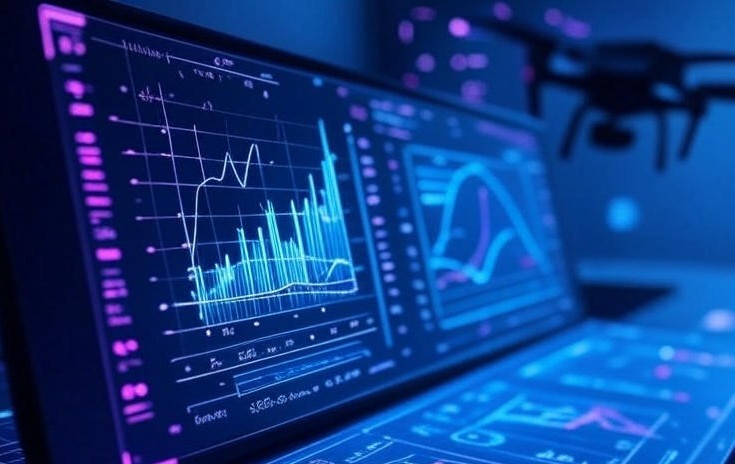
\includegraphics[width=\columnwidth]{images/header-1.jpg}
\end{adjustbox}
%-----------------------------------------------------------------
% initial version - overfull hbox
%-----------------------------------------------------------------
% \colorbox{RoyalBlue}{
% 	\textcolor{white}
% 	{\makebox[\linewidth][c]{\LARGE{\textbf{
% 					Model Predictive Control
% 				}}}}}
% \colorbox{lightgray}{\textcolor{Black}
% 	% \colorbox{BrickRed}{\textcolor{White}
% 	{\makebox[\linewidth][c]{\normalsize{
% 				\textbf{Silvan Stadelmann}
% 				- \selectlanguage{german}{\today}
% 				- v0.1.0
% 				% \url{silvasta@ethz.ch}
% 			} }}}
% \begin{center}
% 	\vspace{-1mm}
% 	{\scriptsize\url{github.com/silvasta/summary-mpc}}
% 	% 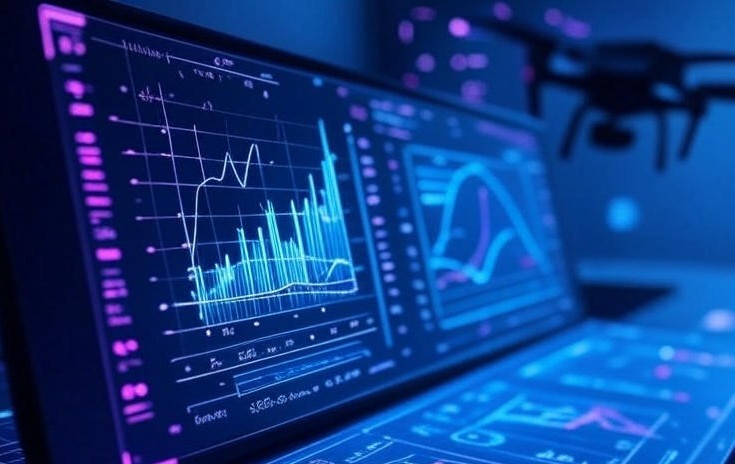
\includegraphics[width=.85\columnwidth]{images/header-1.jpg}
% 	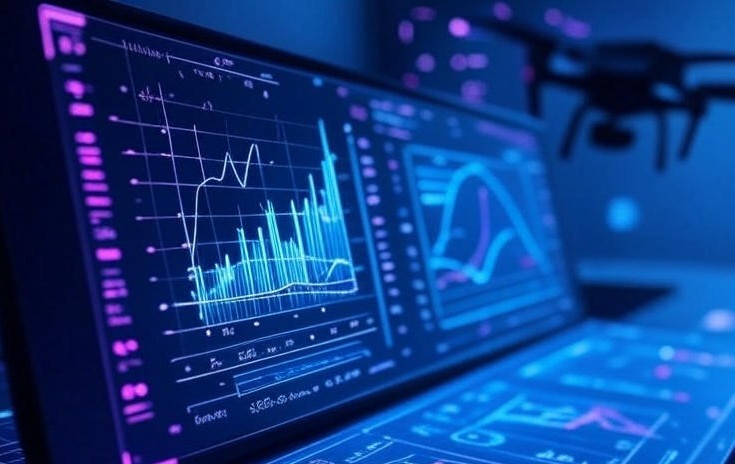
\includegraphics[width=\columnwidth]{images/header-1.jpg}
% \end{center}




		%-----------------------------------------------------------------
		\iftoggle{use-small-font}{\footnotesize}{}
		%-----------------------------------------------------------------
		\renewcommand{\contentsname}{}
		\vspace{-5mm}
		\begin{spacing}{0.9}
			\tableofcontents
		\end{spacing}
		%-----------------------------------------------------------------
		
\begin{sstTitleBox}[BrickRed]{
		Requirements and Steps to MPC
	}
	\begin{centering}
		\begin{sstOnlyFrame}[BrickRed]
			\small
			\ssthl{ 1 }
			\textbf{Model of the System}
			dynamics to state space

			\ssthl{ 2 }
			\textbf{State Estimator}
			track trajectory and disturbance

			\ssthl{ 3 }
			\textbf{Optimal Control Problem}
			define strategy

			\ssthl{ 4 }
			\textbf{Optimization problem}
			mathematical formulation

			\ssthl{ 5 }
			\textbf{Get Optimal Control Sequenc}
			solve optimization

			\ssthl{ 6 }
			\textbf{Verify Closed-Loop Performance}
			iterative tests
		\end{sstOnlyFrame}
	\end{centering}
\end{sstTitleBox}

		% \vfill\null
		% \columnbreak
		%-----------------------------------------------------------------
		\section{Introduction to Systems and Controls}
		

\subsection{Exact ODE Solution of a Linear System}

\textbf{Idea}
Create a model by solving the systems physical equations

\[
	x(t) = e^{A^c(t-t_0)}x_0 +
	\textstyle\int_{t_0}^{t}e^{A^c(t-\tau)}B^c u(\tau)d\tau
\]

\textbf{Problem}
Most physical systems are nonlinear

\textbf{Trick}
First Order Taylor expansion
$f(\bar{x}) + \left. \frac{\partial f}{\partial x^\top} \right
	\rvert_{\bar{x}} (x-\bar{x})$

\subsection{Linearization}
\textbf{Idea}
Nonlinear system  stable enough around an equilibrium

\begin{minipage}[t]{0.5\linewidth}
	\vspace{1mm}
	\begin{align*}
		\dot{x_s}      & =g(x_s,u_s) = 0             \\ \\
		y_s            & = h(x_s,u_s)                \\
		\\
		\Delta \dot{x} & =\dot{x} -\dot{x_s}         \\
		               & = A^c\Delta x + B^c\Delta u \\ \\
		\Delta y       & = y - y_s                   \\
		               & = C\Delta x + D\Delta u
	\end{align*}
\end{minipage}
\begin{minipage}[t]{0.4\linewidth}
	\begin{align*}
		A^c  = \left.\frac{\partial g}{\partial x^T}\right|
		_{\substack{x_s \\u_s}}\\
		B^c  = \left.\frac{\partial g}{\partial u^T}\right|
		_{\substack{x_s \\u_s}}\\
		C    = \left.\frac{\partial h}{\partial x^T}\right|
		_{\substack{x_s \\u_s}}\\
		D    = \left.\frac{\partial h}{\partial u^T}\right|
		_{\substack{x_s \\u_s}}\\
	\end{align*}
\end{minipage}

\subsection{Discretization}

For general nonlinear systems only approximate discretization methods
exist, such as Euler, quality depends on sampling time

\begin{minipage}[t]{0.5\linewidth}
	\textbf{Approximation}\\
	\[
		\dot{x}^c \approx \frac{x^c(t + T_s)-x^c(t)}{T_s}
	\]
\end{minipage}
\begin{minipage}[t]{0.45\linewidth}
	\textbf{Notation}

	$x(k):= x^c(t_0+kT_s)$\\
	$u(k):= u^c(t_0+kT_s)$\\
\end{minipage}

\textbf{Exact Discretization of Linear Time-Invariant Models}

\begin{align*}
	x(t_{k+1}) & =
	\underbrace{e^{A^c T_s}}
	_{=A} x(t_k) +
	\underbrace{\textstyle\int_{0}^{T_s}
		e^{A^c(T_s - \tau)}B^c d\tau}
	_{B=(A^c)^{-1}(A-I)B^c} u(t_k)
	\\
	x(k+N)     & = A^N x(k) + \textstyle\sum_{i=0}^{N-1}
	A^i B u(k+N-1-i)
\end{align*}

\subsection{Analysis of LTI Discrete-Time Systems}

\textbf{Controllabe}
$
	\text{if rank}(\mathcal{C}) = n
	,\;
	\mathcal{C} =
	\begin{bmatrix}
		B & \cdots & A^{n-1} B
	\end{bmatrix}
$

$\forall(x(0),x^*)\exists$ finite time $N$
with inputs $\mathcal{U}$, s.t. $x(N)=x^*$

\textbf{Stabilizable} iff all uncontrollable modes stable

\textbf{Observable}
$
	\text{if rank}(\mathcal{O}) = n
	,\;
	\begin{bmatrix}
		C^\top & \cdots & (CA^{n-1})^\top
	\end{bmatrix}^\top
$

$\forall x(0)\exists$ finite time $N$, s.t. the measurements

$y(0), \dots, y(N-1)$
uniquely distinguish initial state $x(0)$

\textbf{Detectable} iff all unobservable modes stable


		
\subsection{Lyapunov}

\begin{sstTitleBox}[Plum]{\center\textbf{\large
			Lyapunov
		}}

	\begin{sstOnlyFrame}[Plum]
		\textbf{Stability} is a property of an
		\textbf{equilibrium point} $\bar{\mathbf{x}}$
		of a system
	\end{sstOnlyFrame}

	\begin{sstOnlyFrame}[Plum]
		\begin{definition}[Lyapunov Stability]
			$\bar{\mathbf{x}}$ is \textbf{Lyapunov stable} if:

			$\forall\ \epsilon>0\ \exists\ \delta(\epsilon)$ s.t.
			$| x(0) - \bar{x} |_{\scriptscriptstyle 2}< \delta(\epsilon) \to
				| x(k) - \bar{x}|_{\scriptscriptstyle 2} < \epsilon$
		\end{definition}
	\end{sstOnlyFrame}

	\begin{sstOnlyFrame}[Plum]
		\begin{definition}[Globally asymptotic stability]
			If $\bar{\mathbf{x}}$ is attractive, i.e.,
			$\lim_{k\to\infty} ||x(k)-\bar{x}||=0,\ \forall x(0)$
			and Lyapunov stable
			then $\bar{\mathbf{x}}$ is \textbf{globally asymptotically stable}.
		\end{definition}
	\end{sstOnlyFrame}

	\begin{sstOnlyFrame}[Plum]
		\begin{definition}[Global Lyapunov function]
			For the equilibrium $\bar{\mathbf{x}}=0$
			of a system $x(k+1)=g(x(k))$,
			a function $V$, continuous at the origin,
			finite and such that
			$\forall\ x\in \mathbb{R}^{n}$:
			\[
				|x|   \to\infty              \Rightarrow V(x)  \to\infty\]
			\[
				V(x)=0 \ \text{ if }\ x=0 \quad\text{else}\quad V(x)>0             \]
			\[
				V(g(x)) - V(x) \leq -\alpha(x)                          \]
			\[
				\text{for continuous positive definite }
				\alpha:\mathbb{R}^n\to \mathbb{R}
			\]

			then  $V:\mathbb{R}^n\to \mathbb{R}$
			is called \textbf{Lyapunov function}.
		\end{definition}
	\end{sstOnlyFrame}

	\begin{sstOnlyFrame}[Plum]
		\begin{theorem}
			%TODO: non linear system (1)
			If a system admits a Lyapunov function $V(x)$,
			then $\bar{\mathbf{x}} = 0$ is
			\textbf{globally asymptotically stable}.
		\end{theorem}
	\end{sstOnlyFrame}

	%WARN: Lyapunov, DIRECT?, indirect, check  L15.p11

	\begin{sstOnlyFrame}[Plum]
		\begin{theorem}[Lyapunov indirect method]
			System linearized around $\bar{\mathbf{x}}=0$
			with resulting matrix $A$ and eigenvalues $\lambda_i$.

			If	$\forall |\lambda_i| < 1$
			then the origin is asymptotically stable.

			if $\exists |\lambda_i| > 1$
			then origin is unstable.

			If $\exists |\lambda_i| = 1$
			we can't conclude anything about stability.
		\end{theorem}
	\end{sstOnlyFrame}

	\begin{sstOnlyFrame}[Plum]
		\begin{minipage}[c]{0.34\linewidth}
			\textbf{Discrete-Time}

			\textbf{Lyapunov equation}
		\end{minipage}
		\begin{minipage}[b]{0.64\linewidth}
			\[A^TPA-P=-Q,\quad Q>0\]
		\end{minipage}
	\end{sstOnlyFrame}

	\begin{sstOnlyFrame}[Plum]
		\begin{theorem}[Existence of solution, DT Lyapunov equation]
			The discrete-time Lyapunov equation has a unique solution
			$P > 0$ iff $A$ has all eigenvalues inside the unit circle,
			i.e. iff the system $x(k+1) = Ax(k)$ is stable.
			%NOTE: remove one iff? Lyapunov existence of suluteion
		\end{theorem}
	\end{sstOnlyFrame}
\end{sstTitleBox}

		

%TODO: box for: Unconstrained Finite Horizon Control Problem



\subsection{Unconstrained Finite Horizon Control}


$$\begin{aligned}
		J^\star(x(0)) :=
		\min_U & x_N^\top P x_N +
		\textstyle\sum_{i=0}^{N-1}
		x_i^\top Q x_i + u_i^\top R u_i
		\\
		\text{subject to  }
		       & x_{i+1}                = Ax_i+Bu_i
		\quad i  = 0,\dots,N-1                      \\
		       & x_0                    = x(0)
	\end{aligned}$$

$P\succeq0$, with $P=P^T$
terminal weight

$Q\succeq0$, with $Q = Q^T$
state weight

$R\succ0$, with $R = R^T$
input weight


\subsubsection{Batch Approach}

expresses cost function in terms of $x(0)$ and input sequence $U$

\[ \begin{bmatrix}
		x_0    \\
		x_1    \\
		\vdots \\
		x_N
	\end{bmatrix}
	=
	\begin{bmatrix}
		\mathbb{I} \\
		A          \\
		\vdots     \\
		A^N
	\end{bmatrix}
	x(0) +
	\begin{bmatrix}
		0        & \cdots & 0 \\
		B        & 0      & 0 \\
		AB       & B      & 0 \\
		\vdots   & \ddots & 0 \\
		A^{N-1}B & \cdots & B
	\end{bmatrix}
	\begin{bmatrix}
		u_0    \\
		u_1    \\
		\vdots \\
		u_{N-1}
	\end{bmatrix} \]


$\overline{Q} := \mathop{\mathrm{blockdiag}}(Q,\dots, Q,P)$
\quad
$\overline{R} := \mathop{\mathrm{blockdiag}}(R,\dots, R)$

\textbf{Optimal Input}
(from $\nabla_UJ(x(0),U)=2HU+2F^\top x(0)=0$)
%TODO: maybe derivation?
%WARN: definition S, F unclear
\[ U^\star(x(0)) =
	- \bigl(
	\underbrace{
			(\mathcal{S}^u)^\top \overline{Q} \mathcal{S}^u + \overline{R}
		}_{H\text{(Hessian)}^{-1}}
	\bigr)
	\underbrace{
		(\mathcal{S}^u)^\top \overline{Q}\mathcal{S}^x
	}_ {F^\top}
	x(0)
\]


\textbf{Optimal Cost}

\scalebox{0.97}[1]{$
		\scriptstyle
		J^\star(x(0)) = x(0)^\top (
		\mathcal{S}_x^\top \overline{Q} \mathcal{S}_x
		- \mathcal{S}_x^\top \overline{Q} \mathcal{S}_u
		(\mathcal{S}_u^\top \overline{Q} \mathcal{S}_u
		+ \overline{R})^{-1}
		\mathcal{S}_u^\top \overline{Q} \mathcal{S}_x
		)x(0)$}


\subsubsection{Recursive Approach}

uses dynamic programming to solve problem backwards from $N$

\[\begin{aligned}
		J_j^\star(x(j)) :=
		\min_{U_{j\to N}} & x_N^\top P x_N \!+
		\sum_{i=j}^{N-1}x_i^\top Q x_i + u_i^\top R u_i
	\end{aligned}\]


\begin{minipage}[t]{0.64\linewidth}
	\textbf{From Principle Of Optimality}
	\[
		J_j^\star(x_j) =
		\min_{u_j} I(x_i,u_i) + J_{j+1}^\star(x_{j+1})
	\]
\end{minipage}
\begin{minipage}[t]{0.32\linewidth}
	\textbf{Optimal Cost-To-Go}
	\[
		J_i^\star(x_i) = x_i^\top P_i x_i
	\]
\end{minipage}

\textbf{Optimal Control Policy}
\[
	u_i^\star = F_i x_i =
	-(B^\top P_{i+1}B + R)^{-1}
	B^\top P_{i+1} A \cdot x(i)
\]

\subsubsection{Comparison of Batch and Recursive Approaches}

Batch optimization returns sequence $U^\star(x(0))$
of \textbf{numeric values} depending only on x(0),
dynamic programming yields \textbf{feedback policies}
$u_i^\star = F_i x_i$ depending on each $x_i$.

\subsection{Infinite Horizon LQR}
\begin{sstTitleBox}[ForestGreen]{\center\textbf{\large
			LQR
		}
		% small text
	}

	\[ \begin{aligned}
			J_\infty^\star(x(k))  & = \min \sum_{i=0}^\infty
			x_i^\top Q x_i + u_i^\top R u_i                                   \\
			\mathrm{subj.\ to }\  & x_{i+1} = Ax_i + Bu_i,\quad    x_0 = x(k)
		\end{aligned} \]

	Same u as for finite problem but with ARE
	Constant  Feedback Matrix $F\infty$
	asymptotically stable for.. Q,R,stabi,detect
	%TODO: details  LQR

	%WARN: Lemma  Lyapunov (look at proof)

\end{sstTitleBox}

\textbf{Choice of P}

1. Match infinite solution, use ARE

2. Assume no control needed after N, use Lyapunov Equation %TODO: Lyapunov link
(makes only sense when asymptotically stable, otherwise P not positive definite)

3. set constraint $x_{i+N}=0$

\subsection{Constrained Finite Time Optimal Control
}

\begin{sstTitleBox}[ForestGreen]{\textbf{\large
			CFTOC Problem
		}
	}
	\[
		J(x(k)) = x_N^\top P x_N + \sum_{i=0}^{N-1}x_i^\top Q x_i + u_i R u_i
	\]
	\begin{centering}
		\begin{sstFrame}[ForestGreen]
			\vspace{-1.5mm}
			\color{white}
			\[ \begin{aligned}
					J^\star (x(k)) = & \min_{U}  I_f(x_N) + \sum_{i=0}^{N-1} I(x_{i}, u_{i}) \\
				\end{aligned} \]
			\vspace{-2.5mm}
		\end{sstFrame}
		\[ \begin{aligned}
				\text{s.t} \quad & x_{i+1} = A x_{i} + Bu_{i},\ i = 0,\dots,N-1                                                  \\
				                 & x_{i} \in \mathcal{X},\ u_{i} \in \mathcal{U},\ \mathcal{X}_N \in \mathcal{X}_f, \ x_0 = x(k)
			\end{aligned} \]
		N is the time horizon and X , U, Xf are polyhedral regions
		%TODO: feasible set
	\end{centering}
	%HACK: L4.p9 combine with UCFTOC
\end{sstTitleBox}

\subsubsection{Transform Quadratic Cost CFTOC into QP}

\textbf{Goal}
$\min_{z\in\mathbb{R}^n}
	\textstyle\frac{1}{2}z^\top H z + q^\top z + r
	\quad\text{s.t. }Gz\leq h,\ Az = b$


\subsubsection{Construction of QP without substitution}

\textbf{Idea} Keep state equations as equality constraints

\textbf{Define variable} $z =
	\begin{bmatrix}
		x_1^\top & \dots x_N^\top & u_0^\top & \dots u_{N-1}^\top
	\end{bmatrix}^\top$

\textbf{Equalities} from system dynamics
$x_{i+1} = Ax_i + Bu_i$

\[
	G_{eq} =
	\begin{bmatrix}
		\begin{smallmatrix}
			\mathbb{I}& & & \\
			-A & \mathbb{I} && \\
			&  \ddots & \ddots \\
			&&-A & \mathbb{I}
		\end{smallmatrix}
		 & \vline
		\begin{smallmatrix}
			-B \\
			& \ddots \\
			& &-B
		\end{smallmatrix}
	\end{bmatrix}
	E_{eq} =
	\begin{bsmallmatrix}
		A      \\
		0      \\
		\vdots \\
		0
	\end{bsmallmatrix}
\]

\textbf{Inequalities}
$G_{in}z \leq w_{in} + E_{in}x(k)$ from
$\mathcal{X}   = \{x \mid A_x x \leq b_x\},
	\mathcal{U}   = \{u \mid A_u u \leq b_u\},
	\mathcal{X}_f = \{x \mid A_f x \leq b_f\}$
%TODO: inequality constraint order

\[
	G_{in} =
	\left[
		\begin{array}{l!{\color{RoyalBlue!50}\vrule}l}
			\noalign{\arrayrulewidth=0.1mm}\arrayrulecolor{RoyalBlue!50}
			%
			\begin{smallmatrix}
				0&&&
			\end{smallmatrix}
			 &
			\begin{smallmatrix}
				0&&&
			\end{smallmatrix}
			\\ \hline
			\begin{smallmatrix}
				A_x&&&\\
				&\ddots&\\
				&&		A_x&\\
				&&&		A_f
			\end{smallmatrix}
			 &
			\begin{smallmatrix}
				0\ \ &&&\\
				&\ \ddots\\
				&&\ 0\ &\\
				&&&\ \ 0
			\end{smallmatrix}
			\\ \hline
			\begin{smallmatrix}
				0\ \ &&&\\
				&\ \ddots\\
				&&\ 0\ &\\
				&&&\ \ 0
			\end{smallmatrix}
			 &
			\begin{smallmatrix}
				A_u&&\\
				&\ddots&\\
				&&A_u&\\
				&&&A_u
			\end{smallmatrix}
		\end{array}
		\right]
	%
	w_{in} =
	\begin{bmatrix}
		\noalign{\arrayrulewidth=0.1mm}\arrayrulecolor{RoyalBlue!50}
		\begin{smallmatrix}
			b_x\\
		\end{smallmatrix}
		\\ \hline
		\begin{smallmatrix}
			b_x\\
			\vdots\\
			b_x\\
			b_f\\
		\end{smallmatrix}
		\\ \hline
		\begin{smallmatrix}
			b_u\\
			\vdots\\
			b_u\\
			b_u\\
		\end{smallmatrix}
	\end{bmatrix}
\]
\[
	E_{in} =
	\left[
		\begin{smallmatrix}
			-A_x \\
			0 \\
			\vdots \\
			0 \\
		\end{smallmatrix}
		\right]
\]

\textbf{Cost Matrix} $\bar{H} = \mathrm{diag}(Q,..., Q, P, R,..., R)$

\textbf{Finally the resulting quadratic optimization problem}
\[\begin{aligned}
		J^\star(x(k)) = \min_z  \left[ z^\top \ x(k)^\top \right]
		\left[\begin{smallmatrix} \bar{H} & 0 \\ 0 & Q \end{smallmatrix}\right]
		\left[ z^\top \ x(k)^\top \right]^\top \\
		\text{s.t}
		\quad G_{in}z \leq w_{in} + E_{in}x(k)
		\quad	G_{eq}z = E_{eq}x(k)
	\end{aligned}\]

\subsubsection{Construction of QP with substitution}

\textbf{Idea} Substitute the state equations.

\textbf{Step 1} Rewrite cost  as

\[\begin{aligned}
		J(x(k)) = & UXXXX              \\
		=         & \begin{bmatrix}
			            U^\top & x(k)^\top
		            \end{bmatrix}
		\left[\begin{smallmatrix}
				      H & F^\top \\
				      F & Y
			      \end{smallmatrix}\right]
		\begin{bmatrix}
			U^\top & x(k)^\top
		\end{bmatrix}^\top
	\end{aligned} \]

%WARN: CFTOC with substitution NOT finished, step 1 AND 2

\textbf{Step 2} Rewrite constraints compaclty as $GU\le w+Ex(k)$

\textbf{Step 3} Rewrite constrained problem as
\[\begin{aligned}
		J^\star(x(k)) = \min_U
		                       & \begin{bmatrix}
			                         U^\top & x(k)^\top
		                         \end{bmatrix}
		\left[\begin{smallmatrix}
				      H & F^\top \\
				      F & Y
			      \end{smallmatrix}\right]
		\begin{bmatrix}
			U^\top & x(k)^\top
		\end{bmatrix}^\top                          \\
		\mathrm{subj. \ to \ } & GU \leq w + Ex(k)
	\end{aligned} \]

%HACK: L_p norm, and transform cftoc to LP

%TODO: Receiding horizon control Notation

		%-----------------------------------------------------------------
		\section{Optimization}
		
\subsection{Optimization}

% A mathematical optimization problem is generally formulated as:

\begin{sstTitleBox}[Plum]{\textbf{\large
			Mathematical Optimization Problem
		}}
	\begin{minipage}{0.70\linewidth}
		\begin{sstOnlyFrame}[Plum]
			\textbf{Decision variable} $x  \in \mathbb{R}^{n}$

			\textbf{Objectivce function} $f: \dom(f)\to\mathbb{R}$

			\textbf{Inequality constraints} $g_i$
			$\scriptstyle(i \in \#\text{constraints})$

			\textbf{Equality constraints} $h_i$
			$\scriptstyle(i \in \#\text{constraints})$

			\textbf{Fesabile set}
			$\mathcal{X}\!\!:=\!\!\{x|g(x)\!\!\le\!\!0,\!h(x)\!=\!0\}$
		\end{sstOnlyFrame}
	\end{minipage}
	\begin{minipage}{0.28\linewidth}
		\begin{sstFullFrame}[Plum]
			{\color{white}
				\vspace{-1mm}
				\[ \begin{aligned}
						 & \textbf{minimize }f(x)   \\
						 & \ \ \ \text{subject to:} \\
						 & \ \ \ g_i(x)  \le 0      \\
						 & \ \ \ h_i(x)  = 0
					\end{aligned} \]
				\vspace{-1mm}
			}
		\end{sstFullFrame}
	\end{minipage}

	\begin{sstOnlyFrame}[Plum]
		\textbf{Feasible point}
		$x\in\dom(f)$ with
		$g_i(x)\le 0,\ h_i(x)=0$

		\textbf{Strictly feasible point}
		$x$ with strict inequality
		$g_i(x)<0$

		\textbf{Optimal value}
		$f^\star (\text{or } p^\star)=
			\inf\{f(x)|
			g_i(x)\le0,h_j=0 \}$
		$f^\star=+\infty$: OP infeasible,
		$f^\star=-\infty$: OP unbound below

		\textbf{Optimizer}
		% (is set)
		set:
		$\argmin_{x \in \mathcal{X}} f(x):=
			\{ x\in\mathcal{X}|f(x)=f^\star\}$
	\end{sstOnlyFrame}

	\begin{sstOnlyFrame}[Plum]
		$x^\star$ is a \textbf{Global Minimum} if $f(x^\star)\leq f(x)$

		$x^\star$ is a \textbf{Local Minimum} if
		$\exists\ \epsilon > 0$ s.t.
		$f(x^\star)\leq f(x)$
		$\forall x \in \mathcal{X} \cap B_\epsilon(x^\star)$,
		open ball with center $x^\star$ and radius $\epsilon$
	\end{sstOnlyFrame}
\end{sstTitleBox}
\subsection{Convex Sets}

\begin{definition}[Convex Set]
	Set $\mathcal{C}$ is convex if and only if
	\[\theta x + (1-\theta)y \in \mathcal{C},
		\ \forall\ x,y \in \mathcal{C},
		\ \forall\ \theta \in [0,1]\]
\end{definition}

\begin{definition}[Hyperplanes]
	$\{x \in \mathbb{R}^n \mid a\T x=b\}$
\end{definition}
\begin{definition}[Halfspaces]
	$\{x \in \mathbb{R}^n \mid a\T x\le b\}$

	can be \textbf{open} (strict inequality)
	or \textbf{closed} (non-strict inequality)
\end{definition}

\begin{definition}[Polyhedra] intersection of
	\textbf{finite} number of closed halfspaces:
	polyhedra $\{x\in\mathbb{R}^n\mid A^{q\times n}x\preceq b^{q\times1},
		% C^{r\times n}x=d^{r\times1}
		\}$
\end{definition}

\begin{definition}[Polytope]
	is a \textbf{bounded} polyhedron.
\end{definition}

\begin{definition}[Convex hull]
	for  $\{v_1,...,v_k\}\in \mathbb{R}^{d}$ is:

	co$(\{v_1,...,v_k\}):=
		\{ x|x=\sum_{i}\lambda_iv_i,
		\lambda\ge0, \sum_{i}\lambda_i=1 \}$
\end{definition}

\begin{definition}[Ellipsoid]
	set:
	$\{ x | (x\!-\!x_c)^\top A^{-1}(x\!-\!x_c) \leq 1 \}$
	where $x_c$ is center of ellipsoid,
	$A \succ 0$ (i.e. positive definite)
	(Semi-axis lengths are square roots of eigenvalues of $A$)
\end{definition}

\begin{definition}[Norm Ball]
	$B_r(x):=
		\{\xi\in\mathbb{R}^{n}:|\xi-x|_p<r\}$
	where $p$ defines the $l_p$ norm, $p=\{1|2|..|\infty\}$
\end{definition}

%TODO: norm p1,2,...

\textbf{Intersection}
$\mathcal{C}_1, \mathcal{C}_2$ cv
$\Rightarrow \mathcal{C}_1 \cap \mathcal{C}_2$ convex \textbf{(cv)}

\textbf{Image under affine map}
$\mathcal{C} \subseteq  \mathbb{R}^{n}$ cv
$\Rightarrow \{Ax+b \mid x \in \mathcal{C} \}$ cv

\textbf{Inverse IoaM}
$\mathcal{C} \subseteq  \mathbb{R}^{m}$ cv
$\Rightarrow \{x\in\mathbb{R}^{n} \mid  Ax+b\in\mathcal{C}\}$ cv

\subsection{Convex Functions}

\begin{definition}[Convex Function]
	$f: \mathcal{C}_\text{convex} \to\mathbb{R}$ is convex iff
	\[
		f(\theta x + (1-\theta)y)\le \theta f(x)+ (1-\theta)f(y),
		\ \forall\ x,y \in \mathcal{C},
		\ \forall\ \theta \in [0,1]\]
	$f$ is strictly convex if this inequality is strict.
\end{definition}


\begin{definition}[Epigraph]
	$f:\mathbb{R}^n \rightarrow \mathbb{R}$ cv
	$\Leftrightarrow$
	epi$(f)$ is cv set
	$$\operatorname{epi}(f):=\{(x,t)\in \mathbb{R}^{n+1} | f(x)\le t\}$$
\end{definition}

\textbf{Check Convexity} $f$ is convex if it is
composition of simple convex function
with convexity preserving operations
or if


$f: \mathbb{R}^n \rightarrow \mathbb{R}$ twice differentiable,
$\partial^2f/\partial x^2 \succeq 0\ \forall\ x \in \mathbb{R}^{n}$

$g: \mathbb{R} \rightarrow \mathbb{R}$ with $g(t)=f(x+tv)$
convex in $t\ \forall\ x,v \in \mathbb{R}^{n}$
$\rightarrow f$ convex (restriction to a line)

%NOTE: first, second order convexity

- the point wise maximum of convex functions is convex

- the sum of convex functions is convex

- $f(Ax+b)$ is convex if $f$ is convex

%TODO: Level set sublevel set

%NOTE: Example convex funcions
\subsection{Convex Optimization}
%NOTE:Definition cvOP

\begin{theorem}
	For a convex optimization problem,
	\textbf{any} locally optimal solution is globally
	optimal (local optima are global optima).
\end{theorem}


%TODO: Equivalent OP, Slack

\textbf{Linear Programming}
$ \operatorname{minimize} c\T x
	\text{ s.t. } Ax-b \ge 0,\ x\ge0$

Step 1:
$\mathcal{L}(x,\lambda_1,\lambda_2) =
	c\T x-\lambda_1\T (Ax-b) -\lambda_2\T x,\ \lambda_i \ge0$
%TODO: LP L3.p40
Step 2:
$\underset{x \in \mathcal{\mathbb{R}}^n}{\operatorname{inf}}
	\mathcal{L}=\lambda_1\T b$
, if $c-A\T\lambda_1-\lambda_2=0$, else $-\infty$

Step 3: Dual,
maximize $b\T\lambda$
s.t.
$c-A\T\lambda\ge0,\lambda\ge0$
(again LP)

\textbf{Quadratic Programming}
min ...
%TODO: QP

		%-----------------------------------------------------------------
		\section{Invariance}
		

\begin{definition}[Positively Invariant Set $\mathcal{O}$]
	For an autonomous or closed-loop system,
	the set $\mathcal{O}$ is positively invariant if:
	\[
		x(k)\in\mathcal{O}\Rightarrow
		x(k+1) \in \mathcal{O},
		\quad \forall k \in \{0,1,\dots\}
	\]
\end{definition}

\begin{definition}[Maximal Positively Invariant Set $\mathcal{O}_\infty$]
	A set that contains all $\mathcal{O}$
	is the maximal positively invariant set
	$\mathcal{O}_\infty \subset \mathcal{X}$
\end{definition}

\begin{definition}[Pre-Sets]
	The set of states that
	in the dynamic system $x(k+1) = g(x(k))$
	in one time step evolves into the target set $\mathcal{S}$
	is the \textbf{pre-set} of $\mathcal{S}$
	$\Rightarrow \pre(\mathcal{S}) := \{x\mid g(x)\in \mathcal{S}\}$
\end{definition}

\begin{theorem}[Geometric condition for invariance]
	Set $\mathcal{O}$ is positively invariant set iff
	$\mathcal{O}\subseteq\pre(\mathcal{O})
		\Leftrightarrow
		\pre(\mathcal{O})\cap\mathcal{O} = \mathcal{O}$
\end{theorem}
\begin{proof}
	\textbf{Necessary} if
	$\mathcal{O} \nsubseteq  \mathrm{pre}(\mathcal{O})$,
	then $\exists\bar{x} \in \mathcal{O}$
	s.t $\bar{x} \notin \mathrm{pre}(\mathcal{O})$
	$\leadsto \bar{x}\in\mathcal{O},
		\bar{x}\notin\mathrm{pre}(\mathcal{O})$,
	thus $\mathcal{O}$ not positively invariant

	\textbf{Sufficient} if
	$\mathcal{O}$ not pos invar set,
	then $\exists \bar{x}\in\mathcal{O}$
	s.t $g(\bar{x}) \notin\mathcal{O}$
	$\leadsto \bar{x}\in\mathcal{O},
		\bar{x}\notin\mathrm{pre}(\mathcal{O})$
	thus $\mathcal{O}\notin \mathrm{pre}(\mathcal{O})$
\end{proof}

\begin{lemma}{Invariant Sets from Lyapunov Functions}

	If $V:\mathbb{R}^n \to \mathbb{R}$ is a Lyapunov function
	for $x(k+1) = g(x(k))$, then
	$Y := \{x \mid V(x) \leq \alpha\}$
	is an invariant set for all $\alpha \geq 0$
\end{lemma}
%WARN: Lyapunov invarian Lemma
\begin{proof}
	Lyapunov property $V(g(x)) - V(x) < 0$
	implies that once $V(x(k))\leq \alpha$,
	$V(x(j))<\alpha$,
	$\forall\ j\ge k \rightarrow$ Invariance
\end{proof}

\textbf{Example System}
$x(k+1) = Ax(k)$, $A^\top P A - P \prec 0 \prec P$
and resulting  Lyapunov function
$V(x(k)) = x(k)^\top P x(k)$
% \textbf{Example System}
% $V(x(k)) = x(k)^\top P x(k)$
% Lyapunov function
% for $x(k+1) = Ax(k)$
% with
% $A^\top P A - P \prec 0 \prec P$

\textbf{Goal} Find the largest $\alpha$ s.t the
invarinat set $Y_\alpha \in \mathcal{X}$

$\qquad Y_\alpha := \{x \mid x^\top P x \leq \alpha\}\subset \mathcal{X} := \{x \mid Fx\leq f\}$

Equivalent to $\max_\alpha \alpha \quad \text{s.t. }\
	h_{Y_\alpha}(F_i) \leq f_i \ \forall i \in \{1\dots n\}$

...

USE ELIPSOID
%TODO: Maximum Elipsoid set
\subsection{Control Invariance}


\begin{definition}[Control Invariant Set]
	$\mathcal{C} \subseteq \mathcal{X}$ control invariant if
	$$x(k) \in \mathcal{C} \Rightarrow
		\ \exists u(k) \in \mathcal{U} \text{ s.t }
		g(x(k),u(k))\in\mathcal{C} \ \forall k$$
\end{definition}

\begin{definition}[Maximal Control Invariant Set $\mathcal{C}_\infty$]
	A set that contains all $\mathcal{C}$
	is the maximal positively invariant set
	$\mathcal{C}_\infty \subset \mathcal{X}$

	\textbf{Intuition} For all states in $\mathcal{C}_\infty$
	exists control law s.t constraints are never violated
	$\leadsto$ \textbf{The best any controller could ever do}
\end{definition}

\textbf{Pre-set}
$\pre(\mathcal{S}):=\{x \mid \exists u\in\mathcal{U}
	\text{ s.t } g(x,u) \in \mathcal{S}\}$

Set $\mathcal{C}$ is control invariant iff:
$\mathcal{C}\subseteq\pre(\mathcal{C})
	\Leftrightarrow
	\pre(\mathcal{C})\cap\mathcal{C} = \mathcal{C}$

\begin{sstTitleBox}[BrickRed]{\center\textbf{\large
			Control Law from Control Invariant Set
		}}

	\begin{sstOnlyFrame}[BrickRed]

		\begin{centering}
			Control law $\kappa(x(k))$ will \textbf{guarantee}
			that the system
			with control invariant set $\mathcal{C}$
			satisfies constraints \textbf{for all time} if
			$$x(k+1)=g(x(k),u(k))\to
				g(x,\kappa(x)) \in \mathcal{C} \ \forall x \in \mathcal{C}$$

			We can use this fact to \textbf{synthesize}
			control law $\kappa$

		\end{centering}
		\begin{sstFullFrame}[BrickRed]\color{white}
			\[
				\kappa(x):=\argmin\{f(x,u) \mid g(x,u)\in\mathcal{C}\}
			\]
		\end{sstFullFrame}

		with $f$ as any function (including $f(x,u)=0)$
	\end{sstOnlyFrame}

	\begin{sstOnlyFrame}[BrickRed]
		Does not ensure that system will converge

		Difficult because calculating control invariant sets is hard

		\textbf{MPC} implicitly describes $\mathcal{C}$
		s.t easy to represent/compute
	\end{sstOnlyFrame}
\end{sstTitleBox}


\subsection{Computing Invariant Sets and Pre-sets}


\begin{minipage}{0.53\linewidth}
	\begin{sstFullFrame}[ForestGreen]
		\color{white}
		\begin{algorithmic}
			\State $\Omega_0 \leftarrow \mathcal{X}$
			\Loop
			\State $\Omega_{i+1} \leftarrow \mathrm{pre}(\Omega_i)\cap\Omega_i$
			\If{$\Omega_{i+1}=\Omega_i$}
			\State\Return $\mathcal{O}_\infty = \Omega_i$
			\EndIf
			\EndLoop
		\end{algorithmic}
	\end{sstFullFrame}
\end{minipage}

(Same but much harder for control invariat sets)


\begin{align*}
	\intertext{\textbf{System for Pre-Set Computation}}
	x(k+1)                & = Ax(k) +Bu(k)
	% & \text{dynamics}
	\\
	u(k)\in\mathcal{U}  : & =\{u|Gu\le g\}
	% & \text{constraints}
	\\
	\mathcal{S}:          & = \{x|Fx\leq f\}
	% & \text{set to check}
	\intertext{\textbf{Invariant Pre-Set}}
	\pre(S):              & =  \{x \mid Ax \in S\}                               \\
	                      & =  \{ x \mid FAx \leq f\}                            \\
	\intertext{\textbf{Control Invariant Pre-Set}}
	\pre(S):              & =  \{x \mid\exists u\in\mathcal{U}, Ax+Bu \in S\}    \\
	                      & =  \{x \mid\exists u\in\mathcal{U}, FAx+FBu \leq f\} \\
	                      & =  \left\{x \mid\exists u\in\mathcal{U},
	\begin{bmatrix} FA & FB \\0&G \end{bmatrix}
	\begin{bmatrix} x \\u \end{bmatrix}
	\leq \begin{bmatrix} f \\g \end{bmatrix} \right\}
	\intertext{This is a \textbf{projection} operation}
\end{align*}


		%-----------------------------------------------------------------
		
\begin{sstTitleBox}[ForestGreen]{\center\textbf{\large
			Ricatti Equations
		}
		Jacopo Francesco Riccati
	}

	% \begin{sstTitleBox}[ForestGreen]
	% 	% \vspace{-1.5mm}
	% 	{\color{white}\textbf{RDE} - Riccati Difference Equation}
	%
	% 	\scalebox{0.97}[1]{$
	% 			\scriptstyle
	% 			P_i = A^\top P_{i+1} A
	% 			+ Q - A^\top P_{i+1} B
	% 			(B^\top P_{i+1} B + R)^{-1}
	% 			B^\top P_{i+1} A$}
	% 	% \vspace{-2.5mm}
	% \end{sstTitleBox}

	\begin{sstOnlyFrame}[ForestGreen]
		% \vspace{-1.5mm}
		% \color{white}
		{\textbf{Riccati Difference Equation - RDE} solved recursively}
		\scalebox{0.97}[1]{$
				\scriptstyle
				P_i = A^\top P_{i+1} A
				+ Q - A^\top P_{i+1} B
				(B^\top P_{i+1} B + R)^{-1}
				B^\top P_{i+1} A$}
		% \vspace{-2.5mm}
	\end{sstOnlyFrame}

	\begin{sstOnlyFrame}[ForestGreen]
		% \vspace{-1.5mm}
		% \color{white}
		{\textbf{Algebraic Riccati Equation - ARE} solved analytically}
		{\center$\scriptstyle
				P_\infty = A^\top P_\infty A
				+ Q - A^\top P_\infty B
				(B^\top P_\infty B + R)^{-1}
				B^\top P_\infty A$}
		% \vspace{-2.5mm}
	\end{sstOnlyFrame}

\end{sstTitleBox}

		\section{Optimal Control}
		%-----------------------------------------------------------------
		\section{Nominal MPC}
		

What can go wrong with \textit{standard} MPC?

- No feasibility guarantee, the problem may not have a solution

- No stability guarantee, trajectories may not converge to  origin

\begin{sstTitleBox}{
		MPC Mathematical Formulation
	}
	\begin{sstOnlyFrame}
		\begin{equation}
			\underset U\argmin
			\sum_{i=0}^{N-1} l(x_i,u_i) + l_f(x_N)
			\label{mpc:nominal}
		\end{equation}

		\vspace{-3mm}
		\begin{minipage}[t]{0.67\linewidth}
			\begin{align*}
				\textbf{Constraints}
				\quad
				x_0     & = x(k)            \\
				x_{i+1} & =Ax_i + Bu_i      \\
				x_{i}   & \in \mathcal{X}   \\
				u_i     & \in \mathcal{U}   \\
				x_N     & \in \mathcal{X}_f
			\end{align*}
		\end{minipage}

		$l_f(\cdot) $and$ \mathcal{X}_f$
		are chosen to mimic an infinite horizon.
	\end{sstOnlyFrame}
\end{sstTitleBox}

%TODO: MPC Proof 1,2 L6.p31

\begin{sstTitleBox}[BrickRed]
	{	Stability of MPC - Main Result}

	\ssthl{\small\ Assumptions }
	\begin{sstOnlyFrame}[BrickRed]

		\ssthl{ 1 }
		Stage cost is
		strictly positive and only zero at the origin

		\ssthl{ 2 }
		Terminal set is \textbf{invariant}
		under local control law $\kappa_f(x_i)$:
		\[
			x_{i+1} = Ax_i + B\kappa_f(x_i) \in \mathcal{X}_f
			\ \ \text\forall\  x_i \in \mathcal{X}_f
		\]

		\quad All state and input \textbf{constraints are satisfied} in $\mathcal{X}_f$:
		\[
			\mathcal{X}_f \in X, \kappa_f(x_i) \in U
			\ \ \forall\  x_i \in \mathcal{X}_f
		\]

		\ssthl{ 3 }
		Terminal cost is a continuous
		\textbf{Lyapunov function} s.t.
		\[
			l_f(x_{i+1}) - l_f(x_i) \leq
			- l(x_i, \kappa_f(x_i)) \quad
			\forall x_i \in \mathcal{X}_f
		\]
	\end{sstOnlyFrame}
	\begin{sstOnlyFrame}[BrickRed]
		\begin{theorem}
			Under the previous assumptions, the closed-loop system under the MPC control law $u_0^\star(x)$
			is asymptotically stable and the set $\mathcal{X}_f$
			is positive invariant for
			\[
				x(k+1) = Ax(k) + Bu_0^\star(x(k))
			\]
		\end{theorem}
	\end{sstOnlyFrame}
\end{sstTitleBox}

%HACK: choice of terminal set and cost, mpc nominal L6.p48

\textbf{Finite-horizon MPC may not satisfy constraints for all time!}

\textbf{Finite-horizon MPC may not be stable!}

-	An infinite-horizon provides stability and invariance.

-	Infinite-horizon \textit{faked} by forcing final state
into an invariant set for which there exists
invariance-inducing controller,
whose infinite-horizon cost can be expressed in closed-form.

-	Extends to non-linear systems, but compute sets is difficult!

		%-----------------------------------------------------------------
		\section{Practical MPC}
		
\subsection{Steady-state Target Problem}

- Reference is achieved by the target
state $x_s$ if $z_s = Hx_s = r$

- Target state should be a steady-state,
i.e. $x_s = Ax_s + Bu_s$

\begin{align*}
	\begin{aligned}
		x_s & = Ax_s + Bu_s \\
		z_s & = Hx_s = r
	\end{aligned}
	\ \Longleftrightarrow \
	\begin{aligned}
		\begin{bmatrix}
			\mathbb{I} - A & -B \\
			H              & 0
		\end{bmatrix}
		\begin{bmatrix}
			x_s \\
			u_s
		\end{bmatrix}
		=
		\begin{bmatrix}
			0 \\
			r
		\end{bmatrix}
	\end{aligned}
\end{align*}

$\nexists$ solution
$\rightarrow$
$\min (Hx_s - r)^\top Q_s (H x_s - r)$
(closest $x$ to $r$)

If $\exists$ multiple feasible $u_s$
$\rightarrow$
compute
$\min u_s^\top R_s u_s$
(cheapest)

$$
	\min_U |z_N - Hx_s|_{P_z}^2
	+ \sum_{i=1}^{N-1} | z_i - Hx_s |_{Q_z}^2
	+ | u_i - u_s |_{R}^2
	%WARN: Constraints, do one general for entiry summary
$$

\subsection{Reference Tracking}

\begin{align*}
	\begin{aligned}
		\Delta x & = x - x_s
		\\
		\Delta u & = u - u_s
	\end{aligned}
	\ \Rightarrow \
	\begin{aligned}
		\Delta x_{k+1}
		 & = x_{k+1} -x_s                          \\
		 & = A\Delta x_k + B u_k - (A x_s + B u_s) \\
		 & = A\Delta x_k + B\Delta u_k             \\
	\end{aligned}
\end{align*}

%TODO: Structure delta notation
% + check with linearization for no doubling
% + move to lecture


\begin{align*}
	\begin{aligned}
		G_x  x & \leq h_x \\
		G_u  u & \leq h_u
	\end{aligned}
	\ \Rightarrow \
	\begin{aligned}
		G_x \Delta x & \leq h_x - G_x x_s \\
		G_u \Delta u & \leq h_u - G_u u_s
	\end{aligned}
\end{align*}

%WARN: MPC for Tracking: Convergence, L7.p20

Assume target feasible with $x_s \in \mathcal{X}, u_s \in \mathcal{U}$,
choose terminal weight $V_f(x)$ and constraint $\mathcal{X}_f$ as in regulation case satisfying
\begin{itemize}[leftmargin=1em]
	\item $\mathcal{X}_f \subseteq \mathcal{X}, K x \in \mathcal{U} \quad \forall x \in \mathcal{X}_f$
	\item $V_f(x(k+1)) - V_f(x(k)) \leq -l (x(k), Kx(k)) \quad \forall x \in \mathcal{X}_f$
\end{itemize}
If in addition the target reference $x_s, u_s$ is such that
\begin{itemize}[leftmargin=1em]
	\item $x_s \oplus \mathcal{X}_f \subseteq \mathcal{X}, K\Delta x + u_s \in \mathcal{U}, \quad \forall \Delta x \in \mathcal{X}_f$
\end{itemize}
then CL system converges to target reference
\begin{align*}
	x(k) \to x_s, z(k) = Hx(k) \xrightarrow{k\to\infty}r
\end{align*}

\begin{proof}
	%TODO: proof tracking

	\begin{itemize}[leftmargin = 1em]
		\item Invariance under local ctrol law inherited from regulation case
		\item Constraint satisfaction provided by extra conditions
		      \begin{itemize}
			      \item $x_s \oplus \mathcal{X}_f \subseteq \mathcal{X} \to x\in \mathcal{X} \forall \Delta \in\mathcal{X_f}$
			      \item $K\Delta x + u_s \in \mathcal{U} \forall \Delta x \in \mathcal{X}_f \to u\in\mathcal{U}$
		      \end{itemize}
		\item Fron asympt stability of the regulation problem: $\Delta x (k) \xrightarrow{k\to\infty}0$
	\end{itemize}
\end{proof}

\textbf{Terminal set} use
$\mathcal{X}_f^{\text{scaled}} = \alpha \mathcal{X}_f$
(s.t. constraints satisfied)

\subsection{Reference Tracking without Offset}

\textbf{Approach}
Model the disturbance,
use the measurements and model
to estimate the state and disturbance
and find control inputs that use
the disturbance estimate to remove offset.

\textbf{Augmented Model}
\begin{align*}
	x_{k+1} & = Ax_k + Bu_k + B_d d_k \\
	y_k     & = Cx_k + C_d d_k
\end{align*}
\textbf{Constant disturbance}
$d_{k+1}  = d_k$

Observable iff
$\begin{bsmallmatrix}
		A - \mathbb{I} & B_d \\ C & C_d
		%FIXME: I eye 1, be carful with cost I(x,u) l(x,u)
	\end{bsmallmatrix}$
has full rank $(=n_x + n_d)$

\textbf{Observer For Augmented Model}

$
	\begin{bmatrix}
		\hat{x}_{k+1} \\
		\hat{d}_{k+1}
	\end{bmatrix}
	\!=\!
	\begin{bmatrix}
		A & \hspace{-2mm} B_d       \\
		0 & \hspace{-2mm}\mathbb{I}
	\end{bmatrix}
	\begin{bmatrix}
		\hat{x}_{k} \\
		\hat{d}_{k}
	\end{bmatrix}
	\!+\!
	\begin{bmatrix}
		B \\
		0
	\end{bmatrix}
	\!u_{k}
	+
	\hspace{-.5mm}
	\begin{bmatrix}
		L_x \\
		L_d
	\end{bmatrix}
	\hspace{-.5mm}
	(C\hat{x}_{k} \!+\! C_d \hat{d}_{k}-y_{k})
$


\textbf{Error Dynamics} $\Rightarrow$
choose $L$ s.t error dynamics converge to $0$
\begin{align*}
	\begin{bsmallmatrix}
		x_{k+1} - \hat{x}_{k+1} \\
		d_{k+1} - \hat{d}_{k+1}
	\end{bsmallmatrix}
	= \left(
	\begin{bsmallmatrix}
		A & B_d        \\
		0 & \mathbb{I}
	\end{bsmallmatrix}
	+
	\begin{bsmallmatrix}
		L_x \\
		L_d
	\end{bsmallmatrix}
	\begin{bsmallmatrix}
		C & C_d
	\end{bsmallmatrix}
	\right)
	\begin{bsmallmatrix}
		x_{k} - \hat{x}_{k} \\
		d_{k} - \hat{d}_{k}
	\end{bsmallmatrix}
\end{align*}

\begin{lemma}
	Steady-state of an asym. stable
	observer satisfies:
	\begin{align*}
		\begin{bmatrix}
			A-\mathbb{I} & B \\
			C            & 0
		\end{bmatrix}
		\begin{bmatrix}
			\hat{x}_\infty \\
			u_\infty
		\end{bmatrix}
		=
		\begin{bmatrix}
			-B_d \hat{d}_\infty \\
			y_\infty - C_d \hat{d}_\infty
		\end{bmatrix}
		\ (\text{for }n_y = n_d)
	\end{align*}
	$\Rightarrow$ Observer output $C\hat{x}_\infty + C_d \hat{d}_\infty$ tracks $y_\infty$ without offset
\end{lemma}

\begin{adjustbox}{rndcorners=0.5mm}
	\begin{lstlisting}[style=sst]
def get_next_u(y: Measurement, r: Reference):
    """
    System handler for offset-free tracking
    """
    # approximate state, disturbance
    x, d = estimator(y)
    # find steady state und generate delta
    x_s, u_s = target_selector(x, r, d)
    x_delta = x - x_s
    # call solver with new parameter
    u_delta = mpc_regulator(x_delta, x_s, u_s)
    u = u_delta + u_s

    return u
\end{lstlisting}
\end{adjustbox}

\subsection{Offset-free Tracking}

\textbf{Goal}
Track constant reference:
$Hy(k) = z(k) \to r$, $k\to\infty$

\begin{align*}
	\begin{aligned}
		%TODO: I-A or A-I (doesnt mater but should be same as steady-state)
		x_s & = Ax_s + Bu_s +B_d\hat{d}_\infty  \\
		z_s & = H(Cx_s + C_d\hat{d}_\infty) = r
	\end{aligned}
	% \ \Longleftrightarrow \
	\begin{aligned}
		\begin{bsmallmatrix}
			A-I & B \\
			HC  & 0
		\end{bsmallmatrix}
		\begin{bsmallmatrix}
			x_s \\
			u_s
		\end{bsmallmatrix}
		=
		\begin{bsmallmatrix}
			0 \\
			r-HC_d\hat{d}
		\end{bsmallmatrix}
	\end{aligned}
\end{align*}

%WARN: Tracking, Concept!!!



\begin{theorem}[Offset-free Tracking: Main Result]
	Assuming
	$n_d = n_y$,
	RHC recursively feasible,
	unconstrained for $k \geq j$,
	control law  $\kappa(\cdot)= \kappa(\hat{x}(k),\hat{d}(k),r)$
	and closed loop system
	\begin{align*}
		x(k+1)        = & Ax(k) + B\kappa(\cdot) + B_d d                                 \\
		\hat{x}(k+1)  = & (A + L_x C)\hat{x}(k) + (B_d + L_x C_d)\hat{d}(k)              \\
		                & + B\kappa(\cdot) - L_x y(k)                                    \\
		\hat{d}(k+1)  = & L_d C \hat{x}(k) + (\mathbb{I} + L_d C_d)\hat{d}(k) - L_d y(k)
	\end{align*}
	converges, then $z(k) = Hy(k) \to r$
	as $k\to\infty$
\end{theorem}

% \subsection{Enlarging the Feasible Set}

%TODO: MPC without Terminal Set

% 
% \usepackage{pstricks}
% \usepackage{pgfplots}
% \usepackage{tikz}
\usetikzlibrary{
	shapes.geometric,
	arrows,
	backgrounds,
	positioning,
	arrows.meta
}

% remove indent
\let\svtikzpicture\tikzpicture
\def\tikzpicture{\noindent\svtikzpicture}

% Defining styles for blocks
\tikzset{
	block/.style 2 args = {
			rectangle,
			font=\small\bfseries\color{#2},
			% draw=white,
			draw=black,
			line width = 0.18mm,
			fill=#1,
			text width=16mm,
			text centered,
			rounded corners = 0.5mm,
			minimum height=10mm
		},
	block/.default = {RoyalBlue}{white}
}

\tikzset{
	sum/.style ={draw,circle,fill=white,minimum size = 1mm}
}

\tikzset{
	dot/.style = {circle, fill, minimum size=#1,
			inner sep=0mm, outer sep=0mm},
	dot/.default = {0.7mm}
}

\begin{tikzpicture}[auto,
		framed, rounded corners=0.5mm,inner frame xsep = 0.4mm,outer frame sep = 0mm,
		background rectangle/.style= {fill=lightgray},
		% background grid/.style={thin, draw=gray,step=1mm}, show background grid
		% background grid/.style={draw=black,step=5mm}, show background grid
	]

	\node [rectangle](title)[
		% font=\small\bfseries\color{black},
		draw=black,
		line width = 0.25mm,
		anchor=north east,
		fill=white,
		text width=16mm,
		inner sep = 0mm,
		rounded corners = 0.5mm,
		minimum height=10mm
	] at (32mm,18mm) {};
	\node (tracking)[font=\small\bfseries\color{black},
		anchor=east,] at (31.5mm,15mm) {TRACKING};
	\node (mpc)[font=\large\bfseries\color{black},
		anchor=east,] at (31.5mm,11mm) {MPC};

	\node [coordinate] (input) at (-35mm,0mm){};
	\node [coordinate] (output) at (35mm,0mm) {};
	\node [block] (t) at (-21mm,0mm){TARGET SELECTOR};
	% \node [block={black}{black}] (t) at (-21mm,0mm){TARGET SELECTOR};
	\node [sum] (x_sum) at (-9mm, 8mm) {};
	\node [dot] (x_s) at (-21mm,8mm){};
	\node at (x_sum.center){\small $\mathbf-$};
	\node [block] (o) at (4mm,15mm) {OPTIMIZER};
	\node [coordinate](o1)[above = 2mm of o.west]{};
	\node [coordinate](o2)[below = 2mm of o.west]{};
	\node [block] (e) at (-6mm,-15mm) {ESTIMATOR};
	\node [coordinate](e1)[above = 2mm of e.east]{};
	\node [coordinate](e2)[below = 2mm of e.east]{};
	\node [coordinate](e_out_1)[above = 2mm of e.west]{};
	\node [coordinate](e_out_2)[below = 2mm of e.west]{};
	\node [sum] (u_sum) at (4mm, 0mm){};
	\node at (u_sum.center){\small $\mathbf+$};
	\node [dot] (u_s) [left = 4mm of u_sum]{};
	\node [dot] (u_to_e) [right = 1mm of u_sum]{};
	\node [block] (p) at (20mm,0mm){PLANT};
	\node [dot] (y_to_e) [right = 2mm of p.east]{};

	% Arrows
	\draw [-Stealth,thick] (input) -- node {$r$} (t);

	\draw [-Stealth,thick] (t) -- node[below,pos=.6] {$u_s$} (u_sum);
	\draw [-Stealth,thick] (u_sum) -- node {$u$} (p);
	\draw [-Stealth,thick] (u_to_e) |- node[right , pos=0.3] {$u$} (e1);

	\draw [-Stealth,thick] (e.north-|x_sum.south) -- node[pos=0.2,right]  {$\hat{x}$} (x_sum);
	\draw [-Stealth,thick] (x_sum) |- node[left=-1mm]  {$\Delta x$}  (o2);
	\draw [-Stealth,thick] (x_s) -- node {$x_s$} (x_sum);
	\draw [-Stealth,thick] (t) |- node[above=.8mm, pos=.8,inner sep = 0mm] {$x_s$} (o1);

	\draw [-Stealth,thick] (o.south-|u_sum.north) -- node[pos=0.3] {$\Delta u$}  (u_sum);
	\draw [Stealth-,thick] (o.south-|u_s.north) -- node {} (u_s);

	\draw [-Stealth,thick] (p) -- node {$y$}(output);
	\draw [-Stealth,thick] (y_to_e) |- node[above,pos=.8]{$y$} (e2);
	\draw [-Stealth,thick] (e_out_2) -| node[left, pos=0.8 ] {$\hat{d}$} (t);
	\draw [-Stealth,thick,color=gray,dashed] (e_out_1) --node[pos=0.6] {\color{gray}$x,..$}  (e_out_1-|input);

\end{tikzpicture}

\subsection{Soft Constraints}

Input constraints are dictated by physical constraints on
the actuators and are usually hard

- State/output constraints arise from practical restrictions
on the allowed operating range and are \textbf{rarely hard}

- Hard state/output constraints always lead to
\textbf{complications in the controller implementation}
%TODO: summarize soft constraints intro text

\begin{sstTitleBox}[ForestGreen]{\center\textbf{\large
			Soft Constrained MPC Problem Setup
		}
		% small text
	}

	% \begin{adjustbox}{rndcorners=0.5mm}
	% 	\begin{sstOnlyFrame}[ForestGreen]
	% 		$
	% 			\min\sum_{i=0}^{N-1}
	% 			x_i^\top Q x_i + u_i^\top R u_i+
	% 		$
	% 		\textcolor{hltext}{\hl{$l_\epsilon(\epsilon_i)$}}
	% 		% +l_\epsilon(\epsilon_i)
	% 		$
	% 			+x_N^\top P x_i+
	% 		$
	% 		% +l_\epsilon(\epsilon_N)
	% 		% $
	% 		\textcolor{hltext}{\hl{$l_\epsilon(\epsilon_N)$}}
	% 	\end{sstOnlyFrame}
	% \end{adjustbox}

	\begin{adjustbox}{rndcorners=0.5mm}
		\begin{sstOnlyFrame}[ForestGreen]
			\[
				\min_u\sum_{i=0}^{N-1}
				x_i^\top Q x_i + u_i^\top R u_i
				+\color{BrickRed}l_\epsilon(\epsilon_i)\color{black}
				+x_N^\top P x_i
				+\color{BrickRed}l_\epsilon(\epsilon_N)
			\]
		\end{sstOnlyFrame}
	\end{adjustbox}
	\[\begin{aligned}
			\text{subj.\ to }\   x_{i+1}      & = Ax_i + Bu_i      \\
			H_xx_i                            & \le k_x+\epsilon_i \\
			H_uu_i                            & \le k_u            \\
			\text{slack variable }	\epsilon_i & \ge0
		\end{aligned}\]

\end{sstTitleBox}

\textbf{Quadratic penalty}
$l_\epsilon(\epsilon_i) =
	\epsilon_i^\top S \epsilon_i$ (e.g $S = Q$)

\textbf{Linear Penalty}
$v|\epsilon_i|_{1/\infty}$

%TODO: mathematical formulation slack

\textbf{Requirement on $l_\epsilon(\epsilon)$}
If the original problem has a feasible solution $z^\star$,
then the softened problem should have the same solution $z^\star$,
and $\epsilon = 0$.

\begin{theorem}[Exact Penalty Funtcion]
	$l_\epsilon(\epsilon) = v \cdot \epsilon$ satisfies requirement for any $v > \lambda^\star \geq 0$,
	where $\lambda^\star$ is optimal Lagrange multiplier for original problem
\end{theorem}

%HACK: Simplification: Separation of Objectives

%NOTE: summary for lecture

		%-----------------------------------------------------------------
		\section{Robust MPC}
		
\textbf{Uncertain System}
$x(k+1) = g(x(k), u(k), w(k); \theta)$

%TODO: Examples of uncertain models

\subsection{Robust Invariance}

\begin{definition}[Robust Positive Invariant Set $\mathcal{O}^\mathcal{W}$]
	For the autonomous system
	$x(k+1)=g(x(k),w(k))$,
	the set $\mathcal{O}^\mathcal{W}$
	is robust positive invariant
	if:
	\[
		x\in\mathcal{O}^\mathcal{W}\Rightarrow
		g(x,w) \in \mathcal{O}^\mathcal{W},
		\quad \forall w \in \mathcal{W}
	\]
\end{definition}

Given set $\Omega$ and dynamic system $x(k+1) = g(x(k), w(k))$,
\begin{align*}
	\mathrm{pre}^{\mathcal{W}}(\Omega) := & \{x \mid g(x,w)\} \in \Omega \ \forall w \in \mathcal{W}
\end{align*}

%WARN: Robust  pre set  to pre set 

\begin{definition}[Robust Pre-Sets]
	The set of states that
	in the dynamic system $x(k+1) = g(x(k),w(k))$
	for all disturbance $w\in\mathcal{W}$
	in one time step evolves into the target set $\Omega$
	is the \textbf{pre-set} of $\Omega$
	$\Rightarrow \pre^\mathcal{W}(\Omega) :=
		\{x|g(x,w)\in \Omega\ \forall w\in\mathcal{W}\}$
\end{definition}

\textbf{Computing Robust Pre-Sets for Linear Systems}

System $Ax(k) + w(k)$, set $\Omega:= \{x \mid Fx \leq f\}$
\begin{align*}
	\mathrm{pre}^{\mathcal{W}}(\Omega)
	 & = \{ x \mid FAx + Fw \leq f\}
	\\
	 & = \{ x \mid FAx \leq f- \max_{w\in\mathcal{W}}Fw \}
	\\
	 & = \{ x \mid FAx \leq f -  h_{\mathcal{W}^i}(F) \}
\end{align*}
%TODO: image robust invariant set?
%
where $h_{\mathcal{W}^i}(F)$ is the support function

\begin{theorem}[Geometric condition for robust invariance]
	Set $\mathcal{O}^\mathcal{W}$
	is robust positive invariant iff
	$\mathcal{O}^\mathcal{W} \subseteq
		\pre^\mathcal{W}(\mathcal{O}^\mathcal{W})$
\end{theorem}

%HACK: Conceptual Algorithm Robust Invariance

\begin{definition}[Minkowski Sum]
	For $A, B \subset \mathbb{R}^{n}$,
	the Minkowski Sum is
	$A \oplus B := \{x + y | x \in A, y \in B\}$
\end{definition}
%TODO: Minkowski, Pontryagin move to math, maybe box

\begin{definition}[Pontryagin Difference]
	For $A, B \subset \mathbb{R}^{n}$,
	the Pontryagin Difference is
	$A \ominus B := \{x | x+e \in A, \forall e \in B\}$
\end{definition}

\subsubsection{Impact of Bounded Additive Noise}

\textbf{Defining a Cost to Minimize}
Expected value,
worst case, max W
nominal case w=0

\subsubsection{Robust Constraint Satisfaction}
%WARN: 4 steps, do once for all occurances

The idea: Compute a set of tighter constraints such that if the nominal
system meets these constraints, then the uncertain system will too.
We then do MPC on the nominal system.

Goal: Ensure that constraints are satisfied for the MPC sequence.

Terminal State Constraint

...is called disturbance reachable set,
%TODO: F i = bigplus, formula and notation

\subsection{Open Loop Robust MPC}
\begin{align*}
	\min_U                & \left[ l_f(x_N) + \textstyle\sum_{i=0}^{N-1} l(x_i, u_i) \right]                                    \\
	\mathrm{subj.\ to }\  & x_{i+1} = A x_i + B u_i                                                                             \\
	                      & x_i \in \mathcal{X} \ominus ( \textstyle\bigoplus_{j=0}^{i-1} A^j \mathcal{W} ), \quad
	u_i \in \mathcal{U}                                                                                                         \\
	                      & x_0 = x(k), \quad x_N \in \mathcal{X}_f \ominus ( \textstyle\bigoplus_{j=0}^{N-1} A^j \mathcal{W} )
\end{align*}

\subsection{Closed Loop Robust MPC}

%WARN: again uncertain constrained Linear system
% closed loop predictions, AND mpc L9.p10

\textbf{Idea}
Separate the available control authority into two parts:

1.
$z(k+1)=Az(k)+Bv(k)$
steers
noise-free \textit{nominal} system
to origin

2.
$u_i=K(x_i-z_i)+v_i$
compensates for deviations,
i.e. a \textit{tracking} controller,
to keep the real trajectory
close to the nominal system.

$\Rightarrow$
We fix the linear feedback controller K offline,
and optimize over the nominal inputs $\{v_0,...,v_{N−1}\}$
and nominal trajectory $\{z_0,...,z_N\}$,
which results in a convex problem.

%TODO: error dynamics and uncertain state evolution

\textbf{Minimum Robust Invariant Set}

$F_\infty = \bigoplus_{j=0}^\infty A_K^j \mathcal{W}$,
$F_0 := \{0\}\Rightarrow$
$F_n = F_{n+1} = F_\infty$%TODO: mathcal F

%WARN: Pseudo algorithm

\begin{sstTitleBox}{\subsection{Robust Constraint-Tightening MPC}}
	% \begin{sstTitleBox}{Robust Constraint-tightening MPC}

	\[\begin{aligned}
			\min_{Z,V} \         & \sum_{i=0}^{N-1} l(z_i, v_i) + l_f(z_N)      \\
			\mathrm{subj.\ to}\  & z_{i+1} = Az_i + Bv_i                        \\
			                     & z_i \in \mathcal{X} \ominus \mathcal{F}_i    \\
			                     & u_i \in \mathcal{U} \ominus K(\mathcal{F}_i) \\
			                     & z_N \in \mathcal{X}_f \ominus \mathcal{N}_N  \\
			                     & z_0 = x(k)                                   \\
		\end{aligned}\]

	$F_i := \mathcal{W} \oplus A_K\mathcal{W} \oplus \dots A_K^{i}\mathcal{W}$

	$$\text{Control\ Law}\   u(k) = v_0^\star + K(x(k)-z_0) = v_0^\star$$

\end{sstTitleBox}

\textbf{Motivation} can robustly ensure constraint satisfactkon at each time step

\textbf{Note} need terminal set $\mathcal{X}_f$ that is robust invariant under tube controller $K$


\subsection{Robust Tube MPC}

\textbf{Idea}
Ignore noise and plan the nominal trajectory,
bound maximum error at any time with RPI set
$\mathcal{E}: \epsilon_i \in \mathcal{E}  ⇒ \epsilon_{i+1} \in \mathcal{E}$

Ideally $\mathcal{E}$ is selected as the minimum RPI set $F_\infty$

We know that the real trajectory stays ‘nearby’ the nominal one%TODO: xi ∈ zi ⊕ E
because we plan to apply the controller%TODO: ui = K (xi − zi ) + vi
in the future
(we won’t actually do this, but it’s a valid sub-optimal plan)

We must ensure that all possible state trajectories satisfy the constraints
This is now equivalent to ensuring that %TODO: zi ⊕ E ⊂ X
(address input constraints later)

%WARN: Pretext Tube

What do we need to make this work?

- Compute the set E that the error will remain inside

Previously we wanted the \textbf{maximum robust invariant set}, or the largest set in
which our terminal control law works.

We now want the \textbf{minimum robust invariant set}, or the smallest set that the
state will remain inside despite the noise.

- Modify constraints on nominal trajectory $\{z_i\}$

$x_i \in z_i \oplus \mathcal{E} =
	\{z_i + e | e \in \mathcal{E}\}$

- Formulate as convex optimization problem

BOX

... and then prove that

- Constraints are robustly satisfied

- The closed-loop system is robustly stable


\begin{sstTitleBox}[BrickRed]{\textbf{\large
			Tube MPC
		}
		% small text
	}

	\[\begin{aligned}
			\text{Feasible set:}  & \quad
			\mathcal{Z}(x_0):=
			\begin{cases}
				z_{i+1} & = Az_i+Bv_i                         \\
				z_i     & \in \mathcal{X}\ominus\mathcal{E}   \\
				v_i     & \in \mathcal{U}\ominus K\mathcal{E} \\
				z_N     & \in \mathcal{X}_f                   \\
				x_0     & \in z_0\oplus\mathcal{E}            \\
			\end{cases}
			\\
			\text{Cost function:} & \quad
			J(Z,V):=\sum_{i=0}^{N-1}
			l(z_i,v_i)+l_f(z_N)
			\\
			\text{Optimization:}  & \quad
			(V^\star(x_0),Z^\star(x_0))=  \\
			                      &
			\quad\quad\argmin_{V,Z}\{J(Z,V)|(Z,V)\in\mathcal{Z}(x_0)\}
			\\
			\text{Control law:}   & \quad
			\mu_\text{tube}(x):=
			K(x-z_0^\star(x))+v_0^\star(x)
		\end{aligned}\]

	\begin{centering}
		\begin{sstOnlyFrame}[BrickRed]
			\vspace{-1.5mm}
			\[ \begin{aligned}
					% formula
					\text{Feasible set:}  & \quad
					\mathcal{Z}(x_0):=
					\begin{cases}
						z_{i+1} & = Az_i+Bv_i                         \\
						z_i     & \in \mathcal{X}\ominus\mathcal{E}   \\
						v_i     & \in \mathcal{U}\ominus K\mathcal{E} \\
						z_N     & \in \mathcal{X}_f                   \\
						x_0     & \in z_0\oplus\mathcal{E}            \\
					\end{cases}
					\\
					\text{Cost function:} & \quad
					J(Z,V):=\sum_{i=0}^{N-1}
					l(z_i,v_i)+l_f(z_N)
					\\
					\text{Optimization:}  & \quad
					(V^\star(x_0),Z^\star(x_0))=  \\
					                      &
					\quad\quad\argmin_{V,Z}\{J(Z,V)|(Z,V)\in\mathcal{Z}(x_0)\}
					\\
					\text{Control law:}   & \quad
					\mu_\text{tube}(x):=
					K(x-z_0^\star(x))+v_0^\star(x)
				\end{aligned} \]
			\vspace{-2.5mm}
		\end{sstOnlyFrame}
	\end{centering}

\end{sstTitleBox}

ASSUMPTIONS %WARN: assumptions tube AND general, L9.p36

\begin{theorem}[Robust Invariance of Tube MPC]
	The set $\mathcal{Z} := \{x|\mathcal{Z}(x)\neq \emptyset\}$
	is a robust invariant set of the system
	$x(k+1)= Ax(k)+B\mu_\text{tube}(x(k)) + w(k)$
	subject to the constraints
	$x, u \in \mathcal{X} \times \mathcal{U}$.
\end{theorem}

%TODO: proof tube


\begin{theorem}[Robust Stability of Tube MPC]
	The state $x(k)$ of the system
	$x(k+1)= Ax(k)+B\mu_\text{tube}(x(k)) + w(k)$
	converges  to the  limit of the set $\mathcal{E}$.
\end{theorem}

\textbf{Putting it all together: Tube MPC}

To implement tube MPC:

\textbf{— Offline —}

1. Choose a stabilizing controller $K$
so that $A + BK$ is (Schur) stable

2. Compute the minimal robust invariant set
$E = F_\infty$ for the system
$x(k+1) = (A + BK)x(k) + w(k), w \in \mathcal{W}^1$

3. Compute the tightened constraints
$\bar{\mathcal{X}} := \mathcal{X} \ominus \mathcal{E},
	\bar{\mathcal{U}} := \mathcal{U} \ominus K\mathcal{E}$

4. Choose terminal weight function $l_f$
and constraint $\mathcal{X}_f$
satisfying assumptions* %TODO: insert link to assumptions

\textbf{— Online —}

1. Measure / estimate state $x$

2. Solve the problem
$(V^\star(x_0),Z^\star(x_0))=
	\argmin_{V,Z}\{J(Z,V)|(Z,V)\in\mathcal{Z}(x_0)\}$

3. Set the input to
$u	=	K(x-z_0^\star(x))+v_0^\star(x)$

%NOTE: example tube, offline design

%TODO summary tube TODO summary robust

		%-----------------------------------------------------------------
		\section{Implementation}
		
CFTOC problem is
\textbf{multiparametric quadratic program}
\ssthl{ mp-QP }

Two options to solve it:

- Iterative optimization methods

- Explicit solution


Let $I := {1, . . . , m}$ be the set of constraint indices.
\begin{definition}
	[Active Set]
	$A(x)$ and it's complement $NA(x)$
	\begin{align*}
		A(x) :=  & \{j\in I: G_jz^\star(x) - S_jx = w_j \} \\
		NA(x) := & \{j\in I: G_jz^\star(x) - S_jx < w_j \}
	\end{align*}
\end{definition}

\begin{definition}[Critical Region]
	$CR_A$ is set of parameters $x$ for which set $A\subseteq I$ of constraints $i$ active at the optimum.
	For given $\bar{x} \in \mathcal{K}^\star$ let $(A,NA) := (A(\bar{x}), NA(\bar{X}))$. Then
	\begin{align*}
		CR_A := \{x\in\mathcal{K}^\star : A(x) = A\} \quad \text{(states share active set)}
	\end{align*}
\end{definition}

\textbf{Online evaluation: Point location}

Sequential search

Logarithmic search



\subsubsection{Large Scale Convex Optimization}

\begin{definition}[Lipschitz continuity]
	$q: \mathbb{R}^{n} \rightarrow \mathbb{R}^{m}$
	is Lipschitz with constant $L$ if:
	$|q(x)-q(y)| \le L |x-y| \forall x,y \in \mathbb{R}^{m}$
\end{definition}
\vspace{-4mm}
$$f \text{ is\textbf{ Lipschitz }(Lip) with constant } L
	\Leftrightarrow
	|\nabla f(x)|_2\le L$$
\vspace{-4mm}

\begin{theorem}
	$\mathcal{C} \subseteq \mathbb{R}^{n}$ non-empty closed \textbf{(cl)} convex set, $y \notin \mathcal{C}$
	$\rightarrow \exists\ a \ne 0, b \in \mathbb{R}$
	s.t. $a\T x + b < a\T y + b,
		\forall x \in \mathcal{C}$
\end{theorem}


\begin{definition}[smoothness]
	$f : \mathbb{R}^{n}\rightarrow \mathbb{R}$
	is $L$-smooth \textbf{($L$-sm)} if
	$\nabla f(x)$
	satisfies
	$|\nabla f(x)-\nabla f(y)|\le L|x-y|$
	$\forall x,y \in \mathbb{R}^{n}$
\end{definition}

Taylor
$\rightarrow$
$f(y)\le f(x)+\nabla f(x)\T (y-x) +\frac{L}{2}|x-y|^2$

\begin{definition}[strong convexity]
	$f : \mathbb{R}^{n}\rightarrow \mathbb{R}$
	is $\mu$-strongly convex \textbf{($\mu$-scv)} if
	$f(y)\ge f(x)+\nabla f(x)\T(y-x)+\frac{\mu}{2}|x-y|^2$
	% $\forall x,y \in \mathbb{R}^{n}$
\end{definition}

\textbf{How to find $\mu/L$},
Spectra of Hessian $\nabla^2f$, min/max eigenvalue

\textbf{Gradient Descent}

$x_{k+1}=x_k-T\nabla f(x_k)$
for
$k = (k_0,\dots,k_N)$
given
$x_0,T$


\textbf{Line search}
optimal step
$\nu_t^*=\argmin_{\nu\in\mathbb{R}}f(x_t-\nu\nabla f(x_t))$


\begin{definition}[]
	\textcolor{hltext}{\hl{ $\operatorname{prox}_\mathcal{C}(x)=$
	$\operatorname{argmin}_{y\in\mathcal{C}}\frac{1}{2}|x-y|^2$ }}
	$\mathcal{C}\subset \mathbb{R}^{n}$
\end{definition}

\begin{lemma}
	cl, cv
	$\mathcal{C}\subset \mathbb{R}^{n}$
	$\rightarrow$
	$|\operatorname{prox}_\mathcal{C}(x)-\operatorname{prox}_\mathcal{C}(y)|$
	$\le$
	$|x-y|$
	$\leftarrow$
	$|\operatorname{prox}_\mathcal{C}(x)-\operatorname{prox}_\mathcal{C}(y)|^2$
	$\le$
	$(\operatorname{prox}_\mathcal{C}(x)-\operatorname{prox}_\mathcal{C}(y))\T(x-y)$
\end{lemma}


\textbf{Projected Gradient Descent}

$x_{k+1}=\operatorname{prox}_\mathcal{C}(x_k-T\nabla f(x_k))$,
for $x_0,k_{0..N},T\in(0,2/L)$

\begin{adjustbox}{rndcorners=0.5mm}
	\begin{lstlisting}[style=sst]
def get_next_u(y: Measurement, r: Reference):
    """
    System handler for offset-free tracking
    """
    # approximate state, disturbance
    x, d = estimator(y)
    # find steady state und generate delta
    x_s, u_s = target_selector(x, r, d)
    x_delta = x - x_s
    # call solver with new parameter
    u_delta = mpc_regulator(x_delta, x_s, u_s)
    u = u_delta + u_s

    return u
\end{lstlisting}
\end{adjustbox}

		%-----------------------------------------------------------------
		\iftoggle{do-multicol}{\end{multicols}}{}

\end{document}
